% Standalone figure: Figure 1 method-overview schematic of the dual-gate certified
% inspection pipeline (part image -> frozen backbone -> score -> G1/G2 certificates
% -> three-way route). Symbolic only, no data plotted; terminology and notation
% mirror Section~\ref{sec:gate} and Section~\ref{sec:floor} of the manuscript
% (t_lo/t_hi, alpha_miss/alpha_fr, alpha_min = 1/(n_cal+1), audited-not-certified).
% Rebuilt 2026-07-16 (directive #3): short labels only (full definitions live in the
% caption), simple TikZ icons in place of text-heavy boxes, compact height.
% Compile: pdflatex fig-overview.tex  (see Makefile)
\documentclass[border=1pt]{standalone}
\usepackage[T1]{fontenc}
\usepackage{amsmath,amssymb}
\usepackage{tikz}
\usetikzlibrary{arrows.meta,positioning,calc,shapes.geometric}

% Colorblind-safe qualitative palette (Okabe-Ito subset), reused from
% fig-crcbaseline.tex: blue <-> escaped-defect/auto-pass axis, vermillion <->
% false-reject/auto-reject axis, bluish green <-> deferral.
\definecolor{cEscaped}{HTML}{0072B2}
\definecolor{cFalseReject}{HTML}{D55E00}
\definecolor{cDeferral}{HTML}{009E73}

% ---- small TikZ glyphs (shapes/icons, not text) ----
\newcommand{\iconCamera}[2]{
  \begin{scope}[shift={(#1,#2)}]
    \draw[thick, rounded corners=0.3mm] (-3.2mm,-2mm) rectangle (3.2mm,2mm);
    \draw[thick] (-1.4mm,2mm) rectangle (0.2mm,2.7mm);
    \draw[thick] (0,0) circle (1.4mm);
    \draw[thick] (0,0) circle (0.5mm);
  \end{scope}
}
\newcommand{\iconGear}[2]{
  \begin{scope}[shift={(#1,#2)}]
    \foreach \a in {0,30,...,330}{
      \draw[thick] (\a:2.1mm) -- (\a:3.1mm);
    }
    \draw[thick] (0,0) circle (2.1mm);
    \draw[thick] (0,0) circle (0.9mm);
  \end{scope}
}
\newcommand{\iconCylinder}[2]{
  \begin{scope}[shift={(#1,#2)}]
    \draw[thick] (-3mm,2.2mm) arc (180:360:3mm and 0.9mm);
    \draw[thick] (-3mm,-2.2mm) -- (-3mm,2.2mm);
    \draw[thick] (3mm,-2.2mm) -- (3mm,2.2mm);
    \draw[thick] (-3mm,-2.2mm) arc (180:360:3mm and 0.9mm);
    \draw[thick] (-3mm,2.2mm) arc (180:0:3mm and 0.9mm);
  \end{scope}
}
\newcommand{\iconLock}[3]{
  \begin{scope}[shift={(#1,#2)}]
    \draw[thick, #3] (-2mm,-2mm) rectangle (2mm,0.6mm);
    \draw[thick, #3] (-1.1mm,0.6mm) arc (180:0:1.1mm and 1.6mm);
    \draw[thick, #3, fill=#3] (0,-0.9mm) circle (0.35mm);
  \end{scope}
}
\newcommand{\iconCheck}[3]{
  \begin{scope}[shift={(#1,#2)}]
    \draw[very thick, #3] (-1.7mm,0) -- (-0.3mm,-1.5mm) -- (1.9mm,1.7mm);
  \end{scope}
}
\newcommand{\iconCross}[3]{
  \begin{scope}[shift={(#1,#2)}]
    \draw[very thick, #3] (-1.5mm,-1.5mm) -- (1.5mm,1.5mm);
    \draw[very thick, #3] (-1.5mm,1.5mm) -- (1.5mm,-1.5mm);
  \end{scope}
}
\newcommand{\iconClock}[3]{
  \begin{scope}[shift={(#1,#2)}]
    \draw[thick, #3] (0,0) circle (2mm);
    \draw[thick, #3] (0,0) -- (0,1.3mm);
    \draw[thick, #3] (0,0) -- (1.3mm,-0.2mm);
  \end{scope}
}

\begin{document}
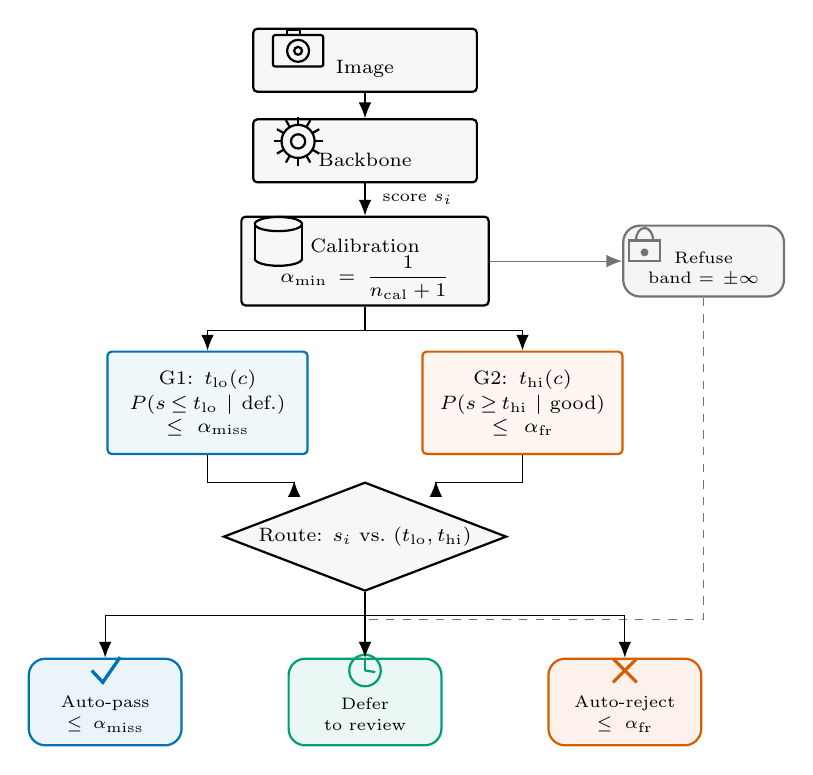
\begin{tikzpicture}[
    font=\fontsize{6.8}{8.1}\selectfont,
    >={Latex[length=2mm,width=1.6mm]},
    every node/.style={align=center},
]

% ---- main pipeline (neutral steps) ----
\node[draw, thick, rounded corners=1.5pt, fill=black!3, minimum height=8mm,
      text width=27mm, inner sep=2pt] (img) at (0,0) {\phantom{x}\\Image};
\iconCamera{-0.85}{0.12}

\node[draw, thick, rounded corners=1.5pt, fill=black!3, minimum height=8mm,
      text width=27mm, inner sep=2pt] (det) at (0,-1.15) {\phantom{x}\\Backbone};
\iconGear{-0.85}{-1.03}

\node[draw, thick, rounded corners=1.5pt, fill=black!3, minimum height=10mm,
      text width=30mm, inner sep=2pt] (cal) at (0,-2.55)
      {\phantom{x}\\Calibration\\$\alpha_{\min}=\dfrac{1}{n_{\text{cal}}+1}$};
\iconCylinder{-1.1}{-2.3}

% ---- refusal branch off the floor check ----
\node[draw, thick, rounded corners=6pt, draw=black!55, fill=black!4,
      minimum height=9mm, text width=19mm, inner sep=2pt,
      font=\fontsize{6.2}{7.4}\selectfont] (refuse) at (4.3,-2.55)
      {\phantom{x}\\Refuse\\band $=\pm\infty$};
\iconLock{3.55}{-2.35}{black!55}

% ---- G1 / G2 certificate gates ----
\node[draw, thick, rounded corners=1.5pt, draw=cEscaped, fill=cEscaped!6,
      minimum height=13mm, text width=24mm, inner sep=2pt] (g1) at (-2.0,-4.35)
      {G1: $t_{\text{lo}}(c)$\\[1pt]
      $P(s\!\le\! t_{\text{lo}}\mid\text{def.})$\\$\le\alpha_{\text{miss}}$};

\node[draw, thick, rounded corners=1.5pt, draw=cFalseReject, fill=cFalseReject!6,
      minimum height=13mm, text width=24mm, inner sep=2pt] (g2) at (2.0,-4.35)
      {G2: $t_{\text{hi}}(c)$\\[1pt]
      $P(s\!\ge\! t_{\text{hi}}\mid\text{good})$\\$\le\alpha_{\text{fr}}$};

% ---- three-way decision ----
\node[draw, thick, diamond, aspect=2.6, fill=black!3,
      inner sep=1pt] (dec) at (0,-6.05) {Route: $s_i$ vs.\ $(t_{\text{lo}},t_{\text{hi}})$};

% ---- outcomes ----
\node[draw, thick, rounded corners=6pt, draw=cEscaped, fill=cEscaped!8,
      minimum height=11mm, text width=18mm, inner sep=2pt,
      font=\fontsize{6.4}{7.6}\selectfont] (pass) at (-3.3,-8.15)
      {\phantom{x}\\[3pt]Auto-pass\\$\le\alpha_{\text{miss}}$};
\iconCheck{-3.3}{-7.75}{cEscaped}

\node[draw, thick, rounded corners=6pt, draw=cDeferral, fill=cDeferral!8,
      minimum height=11mm, text width=18mm, inner sep=2pt,
      font=\fontsize{6.4}{7.6}\selectfont] (defer) at (0,-8.15)
      {\phantom{x}\\[3pt]Defer\\to review};
\iconClock{0}{-7.75}{cDeferral}

\node[draw, thick, rounded corners=6pt, draw=cFalseReject, fill=cFalseReject!8,
      minimum height=11mm, text width=18mm, inner sep=2pt,
      font=\fontsize{6.4}{7.6}\selectfont] (reject) at (3.3,-8.15)
      {\phantom{x}\\[3pt]Auto-reject\\$\le\alpha_{\text{fr}}$};
\iconCross{3.3}{-7.75}{cFalseReject}

% ---- arrows: main pipeline ----
\draw[->] (img) -- (det);
\draw[->] (det) -- node[right, font=\fontsize{6.2}{7.4}\selectfont, xshift=1mm]
      {score $s_i$} (cal);
\draw[->] (cal.south) -- ++(0,-0.3) -| (g1.north);
\draw[->] (cal.south) -- ++(0,-0.3) -| (g2.north);
\draw[->, black!55] (cal.east) -- (refuse.west);
\draw[->] (g1.south) -- ++(0,-0.35) -| ($(dec.north)+(-0.9,0)$);
\draw[->] (g2.south) -- ++(0,-0.35) -| ($(dec.north)+(0.9,0)$);
\draw[->, black!55, dashed] (refuse.south) -- (4.3,-7.1) -- (0,-7.1) -- (defer.north);
\draw[->] (dec.south) -- ++(0,-0.3) -| (pass.north);
\draw[->] (dec) -- (defer);
\draw[->] (dec.south) -- ++(0,-0.3) -| (reject.north);

\end{tikzpicture}
\end{document}
